\begin{frame}{Máximo beneficio}
  \begin{columns}
    \begin{column}{0.5\textwidth}
      $P(x)=5000+1000x-5x^2$, con $a<0$.
      \[ x=-\frac{b}{2a}=100 \]
      \begin{alertblock}{Conclusión}
        Máximo $55000$ en $x=100$.
      \end{alertblock}
    \end{column}
    \begin{column}{0.5\textwidth}
      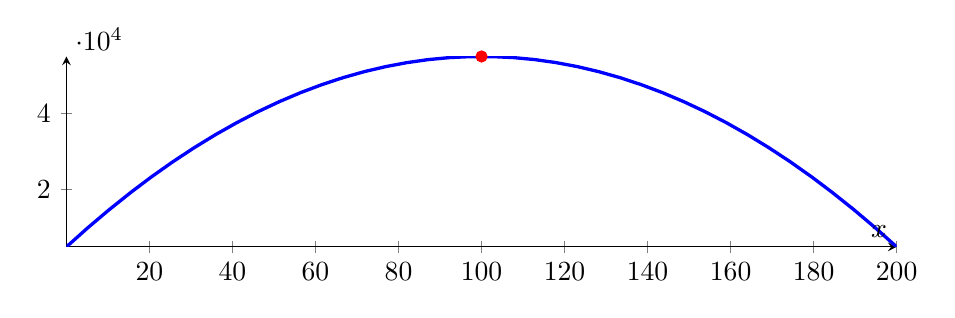
\begin{tikzpicture}
      \begin{axis}[width=\linewidth,height=4cm,
                   axis lines=middle,xlabel=$x$]
        \addplot[blue,very thick,domain=0:200,
                 samples=40]{5000+1000*x-5*x^2};
        \addplot[red,only marks,mark=*]
          coordinates {(100,55000)};
      \end{axis}
      \end{tikzpicture}
    \end{column}
  \end{columns}
\end{frame}
